\chapter{Calibration de la probabilité d'entrer en phase de pupaison} 
\label{chap:pup_chelou}

On s'intéresse ici à une version du modèle qui diffère légèrement de celle décrite dans la partie~\ref{chap:temp}.
On cherche toujours à ajuster la probabilité d'entrer en phase de pupaison en fonction de la température.

On repart de la formule
\[
p_{\text{p}} = 1.9555 - 0.055\times t_{15j},
\]
à laquelle on rajoute la possibilité d'effectuer certaines modifications.
On introduit deux coefficients, $\varpi\in [1; 4]$ et $p_{\text{p}}^*\in [0; 1]$, comme suit :
\[
\widetilde p_{\text{p}} = \left( p_{\text{p}} - \overline{p_{\text{p}}} \right) \times \varpi + p_{\text{p}}^*,
\]
où $\widetilde p_{\text{p}}$ sera la probabilité d'entrer en pupaison et d'y survivre utilisée par le modèle et $\overline{p_{\text{p}}}$ la moyenne de la probabilité de pupaison.
Comme dans la partie \ref{chap:temp}, le coefficient $\varpi$ permet au modèle d'amplifier la variabilité de la probabilité d'entrer en pupaison.
La nouveauté est ici le coefficient $p_{\text{p}}^*$, qui permet au modèle de calibrer la probabilité d'entrer en pupaison moyenne sur la saison.





La figure~\ref{fig:params} montre les valeurs trouvés après calibration pour les deux paramètres présentés ci-dessus.
Et il s'avère qu'il n'y a  que très peu de variabilité pour les deux paramètres, les deux étant très souvant fixés à 1.




\begin{figure}
 \centering
 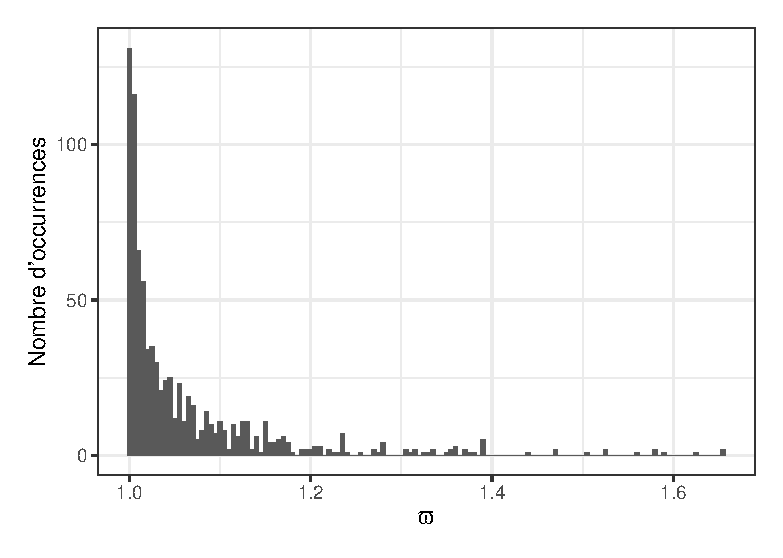
\epsfig{file = plots/varpi.eps, scale = 0.55}
 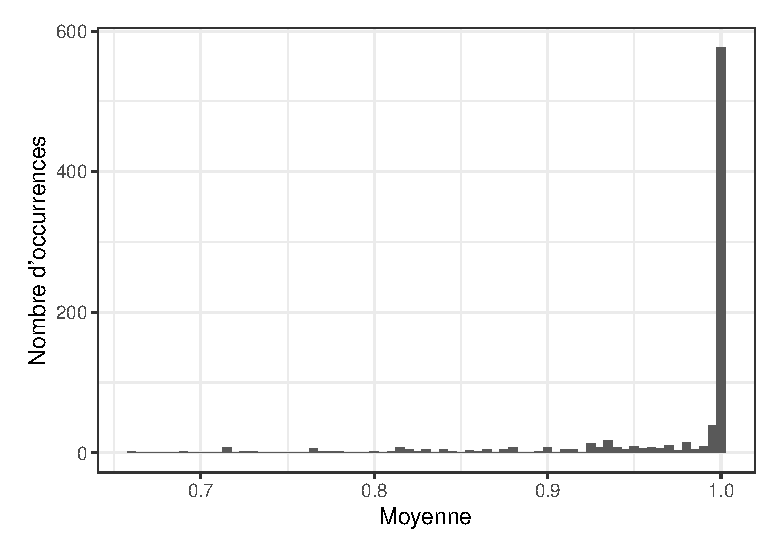
\epsfig{file = plots/intercept.eps, scale = 0.55}
 \caption{Résultats de la calibration pour les paramètres $\varpi$ et $p_{\text{p}}^*$.}
 \label{fig:params}
\end{figure}


Or, comme le montre la figure~\ref{fig:prob}, il en résulte que la probabilité d'entrer en pupaison est quasi-constante.
La seule différence avec le modèle initial est que cette quasi-constante est proche de 1 au lieu de 0.77.

\begin{figure}
 \centering
 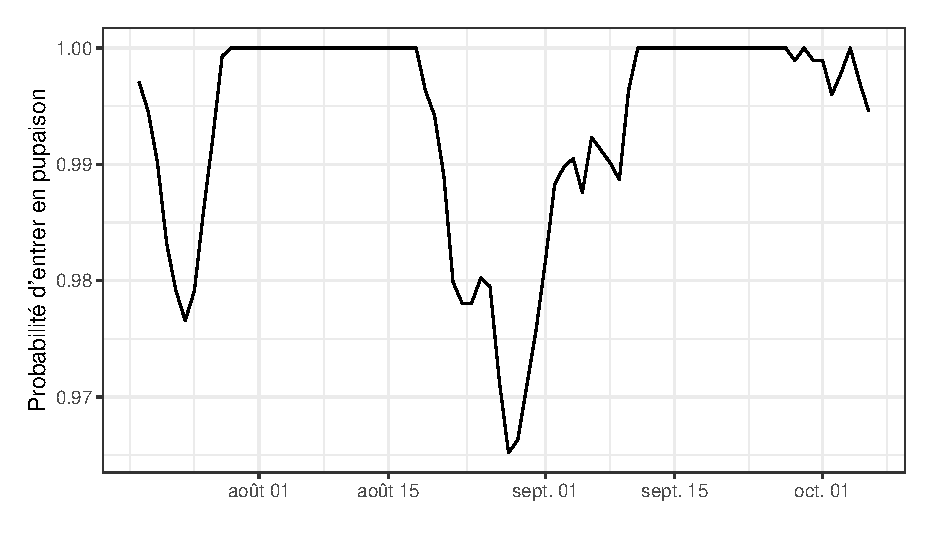
\epsfig{file = plots/pupaison_chelou.eps, scale = 0.7}
 \caption{Probabilité d'entrer en phase de pupaison obtenue lorsque $\varpi = 1$ et $p_{\text{p}}^* = 1$.}
 \label{fig:prob}
\end{figure}

On retrouve, sans surprises, trois solutions--type qui sont très similaires à celles des parties~6.1 et \ref{chap:temp}.
Il apparaît alors peu utile de les afficher.
